\documentclass[12pt]{article}
\usepackage{amsmath}
\usepackage{amsthm}
\usepackage{graphicx,psfrag,epsf}
\usepackage{enumerate}
\usepackage{natbib}
\usepackage{url} % not crucial - just used below for the URL
\usepackage{color}
\usepackage{mathtools}

%\pdfminorversion=4
% NOTE: To produce blinded version, replace "0" with "1" below.
\newcommand{\blind}{0}

% DON'T change margins - should be 1 inch all around.
\addtolength{\oddsidemargin}{-.5in}%
\addtolength{\evensidemargin}{-.5in}%
\addtolength{\textwidth}{1in}%
\addtolength{\textheight}{1.3in}%
\addtolength{\topmargin}{-.8in}%


%%%% Packages and definitions
\usepackage{amssymb}

\usepackage{xr}

\usepackage[top=0.85in,left=1.0in,right=1.0in,footskip=0.75in]{geometry}

% Use adjustwidth environment to exceed column width (see example table in text)
\usepackage{changepage}

% Use Unicode characters when possible
\usepackage[utf8]{inputenc}

% textcomp package and marvosym package for additional characters
\usepackage{textcomp,marvosym}

\usepackage[ruled]{algorithm}
\usepackage{algorithmic}

% cite package, to clean up citations in the main text. Do not remove.
\usepackage{cite}

% Use nameref to cite supporting information files (see Supporting Information section for more info)
\usepackage{nameref,hyperref}

%\usepackage{amsthm}

% ligatures disabled
\usepackage{microtype}
\DisableLigatures[f]{encoding = *, family = * }

% for the beautiful checkmarks
\usepackage{pifont}

\newtheorem{theorem}{Theorem}
\newtheorem{corollary}{Corollary}
\newtheorem{lemma}{Lemma}
\newtheorem{definition}{Definition}
\newtheorem{condition}{Condition}

\DeclareMathOperator*{\argmin}{arg\,min}


\begin{document}

\def\spacingset#1{\renewcommand{\baselinestretch}%
{#1}\small\normalsize} \spacingset{1}


%%%%%%%%%%%%%%%%%%%%%%%%%%%%%%%%%%%%%%%%%%%%%%%%%%%%%%%%%%%%%%%%%%%%%%%%%%%%%%

\if0\blind
{
  \title{\bf Oracle inequalities for validation set procedures with applications to penalized regression}
  \author{Jean Feng\thanks{
    Jean Feng was supported by NIH grants ???. % DP5OD019820 and T32CA206089.
    Noah Simon was supported by NIH grant DP5OD019820.
    The content is solely the responsibility of the authors and does not necessarily represent the official views of the National Institutes of Health.}\\
    Department of Biostatistics, University of Washington\\
    and \\
    Noah Simon \\
    Department of Biostatistics, University of Washington}
  \maketitle
} \fi

\if1\blind
{
  \bigskip
  \bigskip
  \bigskip
  \begin{center}
    {\LARGE\bf title goes here}
\end{center}
  \medskip
} \fi

\bigskip
\begin{abstract}

In the regression setting, model-estimation procedures construct models given training data and a set of hyperparameters. The optimal hyperparameters that minimize the model error are unknown so they are often estimated using validation set approaches. In this paper, we establish finite-sample oracle inequalities for cases where the model-estimation procedures are smoothly parameterized by the hyperparameters. Moreover, in the training/validation split framework, we establish a sharp oracle inequality on the model error, with additional near-parametric terms. Our main application is penalized regression problems with multiple penalty parameters. We establish that tuning penalty parameters only adds a near-parametric-rate error term by showing the fitted models are indeed Lipschitz in the penalty parameters. Hence we show that for semi- and non-parametric problems, the degree of overfitting is relatively small for regression problems with multiple penalty parameters.
\end{abstract}

\noindent%
{\it Keywords:}  Hyperparameter selection, Cross-validation, Regularization, Regression
\vfill

\newpage
\spacingset{1.45}
\section{Introduction}

Per the usual regression framework, we observe response $y \in \mathbb{R}$ and predictors $\boldsymbol {x} \in \mathbb{R}^p$. Suppose $y$ is generated by a true model $g^*$ plus random error $\epsilon$ with expectation zero, as follows
\begin{equation}
\label{true_model}
y = g^*(\boldsymbol x) + \epsilon
\end{equation}
Our goal is to estimate $g^*$.

Many model-estimation procedures can be formulated as selecting a model from some function class $\mathcal{G}$ given training data $T$ and $J$-dimensional hyperparameter vector $\boldsymbol{\lambda}$. For example, in penalized regression problems, the fitted model can be expressed as the minimizer of the penalized training criterion
\begin{equation}
\label{intro_penalized_regression}
\hat{g}(\boldsymbol \lambda | T) = \argmin_{g\in \mathcal{G}} \sum_{(x_i, y_i) \in T} \left (y_i -  g(x_i) \right )^2 + \sum_{j=1}^J \lambda_j P_j(g)
\end{equation}
where $P_j$ are penalty functions and $\lambda_j$ are penalty parameters. As suggested by the notation in \eqref{intro_penalized_regression}, the penalty parameters are the hyperparameters in this model-estimation procedure.

Given a set of possible hyperparameters $\Lambda$, there is some oracle hyperparameter $\tilde{\boldsymbol{\lambda}}$ in $\Lambda$ that minimizes the difference between the fitted model and the true model. Usually $\tilde{\boldsymbol{\lambda}}$ is unknown so it is estimated using training/validation split or cross-validation. The basic idea is to fit models on a random partition of the observed data and evaluate their error on the remaining data. The final hyperparameters $\hat{\boldsymbol{\lambda}}$ are the minimizer of the error on this validation set. For a more complete review of cross-validation, refer to \citet{arlot2010survey}.

The performance of validation set procedures is typically characterized by an oracle inequality that bounds the generalization error of the expected model selected from the validation set procedure. Most approaches suppose that $\Lambda$ is finite.  Finite-sample oracle inequalities have been established for a training/validation framework \citet{gyorfi2006distribution} and a general cross-validation framework \citep{van2003unified, van2004asymptotic}. To handle the case where $\Lambda$ has infinite elements, one can use entropy-based approaches \citep{lecue2012oracle}. 

The goal of this paper is to characterize the performance of models when the hyperparameters must be tuned by some validation set procedure. We are particularly interested in an open question raised in \citet{bengio2000gradient} (and possibly by others): what is the ``amount of overfitting... when too many hyperparameters are optimized''? To do this, we establish finite-sample oracle inequalities of the form
\begin{equation}
\label{thrm:intro_oracle_ineq}
\left \| g^* - \hat{g}\left (\hat{\boldsymbol{\lambda}}, T \right ) \right \|^2
\le
c
\underbrace{\inf_{\lambda \in \Lambda} \left \| g^* - \hat{g}\left (\boldsymbol{\lambda} , T \right ) \right \|^2}_{\text{Oracle error}}
+ \text{ error}
\end{equation}
for some norm $\| \cdot \|$ and constant $c \ge 1$. Under the assumption that the model-selection procedure is smoothly parameterized by the hyperparameters, we find that the error from the model-selection procedure shrinks at roughly a parametric rate. So for semi- and non-parametric regression problems, this term is generally dominated by the oracle error. In these settings, the amount of overfitting is small if the number of hyperparameters is fixed. In fact, the number of hyperparameters can grow without affecting the asymptotic convergence rate.

The main application in this paper is penalized regression models of the form \eqref{intro_penalized_regression}. We show that the fitted model is indeed smoothly parameterized by the penalty parameters so our oracle inequalities apply. Again, we find that additional penalty parameters only add a near-parametric error term, which has a negligible effect on the model error in semi- and non-parametric settings. This result suggests that the recent interest in combining penalty functions (e.g. elastic net and sparse group lasso \citep{zou2003regression, simon2013sparse}) may have artificially restricted themselves to two-component combinations. Adding more penalties may lead to better models.

There seem to be little theoretical results relating the number of hyperparameters to the model error. Most oracle inequalities only consider one-dimensional hyperparameters \citep{lecue2012oracle, van2003unified, van2004asymptotic, gyorfi2006distribution}. Within the context of penalized regression problems, the oracle inequalities are also only for the case of a single penalty parameter \citep{golub1979generalized, chetverikov2016cross, chatterjee2015prediction}. A potential reason for this dearth of literature is that, historically, tuning multiple hyperparameters was computationally difficult. However, there have been many proposals recently for overcoming this computational hurdle \citep{bengio2000gradient, foo2008efficient, snoek2012practical}.

Section \ref{sec:main_results} present oracle inequalities for models selected by training/validation split and cross-validation to elucidate the relationship between the model error and the number of hyperparameters.
Section \ref{sec:examples} applies these results to penalized regression models.
Section \ref{sec:simulations} provides a simulation study to support our theoretical results.
Section \ref{sec:discussion} discusses our findings and potential future work.
Proofs are in Section \ref{sec:proofs}.

\section{Main Result} \label{sec:main_results}

In this section, we establish oracle inequalities for the model error from tuning hyperparameters by  training/validation split and cross-validation.
%The final model is the output of a two step process. First, a set of models are generated using a model-estimation procedure for each hyperparameter vector in $\Lambda \subseteq \mathbb{R}^J$. Then we perform model-selection over this set to get the final model. 
We first introduce some notation and formalize the model-estimation procedure. 

Let $D^{(n)}$ denote a dataset with $n$ samples from the model \eqref{true_model} where $\epsilon$ are independent random variables with expectation zero. Suppose $\epsilon_1,...,\epsilon_n$ are uniformly sub-Gaussian with parameter $b>0$; i.e. $\max_{i=1,...,n} \mathbb{E} e^{t \epsilon_i} \le e^{b^2t^2/2}$ for all $t \in \mathbb{R}$.

The model-estimation procedure accepts some hyperparameter of dimension $J$ and training data of size $m$ to output a fitted model from some model class $\mathcal{G}$. This can be formulated as an operator $\hat{g}^{(m)}(\cdot | D^{(m)})$ that maps a hyperparameter vector $\boldsymbol{\lambda}$ from some set $\Lambda \subseteq \mathbb{R}^J$ to a function in $\mathcal{G}$. 

In this section, we focus on model-estimation procedures that are Lipschitz.
\begin{definition}
	\label{def:smooth_funcs}
	Let $\mathcal{F}$ be a function class. Let $\Lambda \subseteq \mathbb{R}^J$.
	The operator $\hat{f}: \Lambda \mapsto \mathcal{F}$ is $C$-Lipschitz in $\boldsymbol{\lambda}$ with respect to norm $\| \cdot \|$ over $\Lambda$ if
	\begin{equation}
	\left \| \hat{f}(\boldsymbol \lambda) - \hat{f}(\boldsymbol \lambda ') \right \|
	\le
	C \| \boldsymbol \lambda - \boldsymbol \lambda' \|_2 
	\quad
	\forall \boldsymbol \lambda,\boldsymbol \lambda' \in \Lambda
	\label{eq:smooth_funcs}
	\end{equation}
\end{definition}
Under this Lipschitz assumption, we show that the additional error incurred for tuning multiple hyperparameters shrinks at roughly a parametric rate. We hypothesize that many model-estimation procedures are smooth in their hyperparameters -- after all, we are probably most interested in procedures that are well-behaved. More general model-estimation procedures are handled in Section \ref{sec:proofs}.

\subsection{Training/Validation Split}

In the training/validation split framework, the dataset $D^{(n)}$ is randomly partitioned into a training set $T$ and validation set $V$ of sizes $n_T$ and $n_V$, respectively. The selected hyperparameter $\hat{\boldsymbol{\lambda}}$ is the minimizer of the validation loss
\begin{equation}
\label{eq:train_val_lambda}
\hat{\boldsymbol \lambda} = \argmin_{\boldsymbol{\lambda} \in\Lambda} \frac{1}{2} \left \| y-\hat{g}^{(n_T)}( \boldsymbol \lambda | D_T^{(n_T)}) \right \|_{V}^{2}
\end{equation}
where $\| h \|_{V}=\frac{1}{n_V}\sum_{i\in V} h^2(x_i)$ for any function $h$. We now present a sharp finite-sample oracle inequality with respect to the norm $\| \cdot \|_{V}$. The result is a special case of Theorem \ref{thrm:train_val_complicated}.
\begin{theorem}
\label{thrm:train_val}
Let $\Lambda=[\lambda_{\min},\lambda_{\max}]^{J}$ where $0 < \lambda_{\min} < \lambda_{\max}$. Suppose independent random variables $\epsilon_1, ... \epsilon_n$ are uniformly sub-Gaussian with parameter $b$. Suppose there are constants $\sigma, C_\Lambda > 0$ such that for any dataset $D^{(n_T)}$ with $\|\boldsymbol{\epsilon}\|_{D^{(n_T)}} \le \sigma$, $\hat g^{(n_T)}(\boldsymbol{\lambda} |D^{(n_T)})$ is $C_\Lambda$-Lipschitz with respect to $\| \cdot \|_V$ over $\Lambda$. Suppose $n C_\Lambda \lambda_{\max} \ge 1$.

Let 
\begin{equation}
\tilde{\boldsymbol \lambda} = \argmin_{\lambda \in \Lambda} \left \| g^*-\hat{g}^{(n_T)}( \boldsymbol{\lambda} | T) \right \|_{V}^{2}
\end{equation}

Then there is a universal constant $c_0$ and a constant $c>0$ only depending on $b$ such that for all $\delta$ satisfying
\begin{equation}
\delta^{2}
\ge
c \left ( 
\frac{J(c_0 + \log (n C_\Lambda\lambda_{\max}))}{n_{V}}
\vee 
\sqrt{\frac{J(c_0 +\log (n C_\Lambda \lambda_{\max}))}{n_{V}}}\left\Vert g^* - \hat{g}^{(n_T)}( \tilde{\boldsymbol{\lambda}} | T)\right\Vert_{V}
\right )
\end{equation}
we have
\begin{eqnarray*}
	Pr\left(
	\left\Vert g^* - \hat{g}^{(n_T)}( \hat{\boldsymbol{\lambda}} | T) \right\Vert _{V}^2 -
	\left\Vert g^* - \hat{g}^{(n_T)}( \tilde{\boldsymbol{\lambda}} | T) \right\Vert _{V}^2
	\ge\delta^2
	\right )
	&\le& c\exp\left(-\frac{n_{V}\delta^{4}}{
		c^{2}
		\left\Vert g^* - \hat{g}^{(n_T)}( \tilde{\boldsymbol{\lambda}} | T) \right\Vert _{V}^2
	}\right) \\
	&& +c\exp\left(-\frac{n_{V}\delta^{2}}{c^{2}}\right) \\
	&& +c\exp\left (
	-\frac{n_T \sigma^2}{c^2}
	\right )
\end{eqnarray*}

\end{theorem}
For ease of interpretation, we present the result in asymptotic order notation below.
\begin{corollary}
	Under the assumptions given in Theorem \ref{thrm:train_val}, we have
	\begin{eqnarray}
	\left\Vert g^* - \hat{g}^{(n_T)}( \hat{\boldsymbol{\lambda}} | T) \right\Vert _{V}^2 &\le& \left\Vert g^* - \hat{g}^{(n_T)}( \tilde{\boldsymbol{\lambda}} | T) \right \Vert^2_{V}\\
	&& + O_p \left(\frac{J(c_0 + \log (n C_\Lambda\lambda_{\max}))}{n_{V}} \right) \label{eq:asym_train_val_theorem1} \\
	&& + O_p \left(
	\sqrt{
		\frac{J(c_0 + \log (n C_\Lambda\lambda_{\max}))}{n_{V}}
		\left\Vert g^* - \hat{g}^{(n_T)}( \tilde{\boldsymbol{\lambda}}| T) \right \Vert^2_{V}
	}
	\right )
	\label{eq:asym_train_val_theorem2}
	\end{eqnarray}
\end{corollary}
We see that the error of the selected model is bounded by oracle error, a near-parametric term \eqref{eq:asym_train_val_theorem1},  and the geometric mean of the two \eqref{eq:asym_train_val_theorem2}. The latter two terms can be thought of as the error incurred from tuning multiple hyperparameters. We now discuss these two terms in more detail.

We refer to \eqref{eq:asym_train_val_theorem1} as near-parametric since it is roughly equal to $J/n_V$, and parametric regression problems usually have a model error on the order of $J/n$, where $J$ is the parameter dimension and $n$ is the number of training samples. The appearance of this term seems to make intuitive sense. We can think of tuning hyperparameters as the problem of estimating $\tilde{\boldsymbol{\lambda}}$ over the $J$-dimensional parameter space given the validation data as training data.

However, the geometric mean in \eqref{eq:asym_train_val_theorem2} suggests that treating the problem of tuning hyperparameters as a parametric regression problem is an oversimplification. The issue is that the model class $\mathcal{G}(T)$ does not contain the true model $g^*$. The bias term 
\begin{equation}
\left\Vert g^* - \hat{g}^{(n_T)}( \tilde{\boldsymbol{\lambda}}|T) \right \Vert^2_{V}
\end{equation}
not only specifies the minimum validation loss achievable, but it also contributes to the convergence rate.

In the semi- and non-parametric regression setting, the oracle error usually shrinks at a polynomial rate of $n_T^\omega$ where $\omega > -1$. Hence in these problems, the oracle error will dominate both the error terms asymptotically. In fact, Theorem \ref{thrm:train_val} states that the maximum rate that the number of hyperparameters can grow without affecting the asymptotic convergence rate is proportional to 
\begin{equation}
\frac{n_{V}}{c_0 + \log (n C_\Lambda\lambda_{\max})}
\left\Vert g^* - \hat{g}^{(n_T)}( \tilde{\boldsymbol{\lambda}}| T) \right \Vert^2_{V}
\end{equation}
As long as the number of hyperparameters does not grow at this rate, the amount of overfitting is likely minimal.

\subsection{Cross-Validation}

In this section, we give an oracle inequality for $K$-fold cross-validation. Previously, the oracle inequality was with respect to the L2 norm over the validation covariates. We are now interested in the generalization error
\begin{equation}
\left \| g - g^* \right \|^2 = \int \left |g(x) - g^*(x) \right |^2 dx
\end{equation}
The result in this section is an application of the oracle inequality in \citet{lecue2012oracle}.

The problem setup for $K$-fold cross-validation is as follows. Let dataset $D^{(n)}$ be randomly partitioned into $K$ sets, which we assume to have equal size for simplicity. Partition $k$ will be denoted $D_k^{(n_V)}$ and its complement will be denoted $D_{-k}^{(n_T)} = D \setminus D_k^{(n_V)}$. We perform our model-selection procedure over $D_{-k}^{(n_T)}$ for $k=1,...,K$ and select the hyperparameter that minimizes the average validation loss
\begin{eqnarray}
\label{kfold_opt}
\hat{\boldsymbol \lambda} &=& \argmin_{\boldsymbol{\lambda} \in\Lambda} \frac{1}{2K} \sum_{k=1}^K  \left \| y-\hat{g}(\boldsymbol \lambda | D_{-k}^{(n_T)}) \right \|_{D_k^{(n_V)}}^{2}
\end{eqnarray}

In traditional cross-validation, the final model is retrained on all the data with $\hat{\boldsymbol{\lambda}}$. However, bounding the generalization error of the retrained model requires additional regularity assumptions \citep{lecue2012oracle}. We consider the ``averaged version of cross-validation'' instead
\begin{equation}
\label{thrm:avg_cv}
\bar{g}\left ( \hat{\boldsymbol \lambda} \middle | {D^{(n)}} \right ) = \frac{1}{K} \sum_{k=1}^K \hat{g} \left (\hat{\boldsymbol \lambda} \middle | D^{(n_T)}_{-k} \right )
\end{equation}

The following theorem bounds the generalization error of \eqref{thrm:avg_cv}. The more general oracle inequality is in \citet{lecue2012oracle}, which is reproduced in Theorem \ref{thrm:k_fold_complicated}.

\begin{theorem}
\label{thrm:kfold}
Suppose the dataset can be partitioned into $K$ equal-sized sets, where $K \ge 2$. Let $\Lambda = [\lambda_{\min}, \lambda_{\max}]^J$. Suppose independent random variables $\epsilon_1, ... \epsilon_n$ have expectation zero and are uniformly sub-Gaussian with parameter $b$. 
Suppose there is a $G \ge  2$ such that $\sup_{g \in \mathcal{G}} \|g\|_\infty \le G$.

Suppose there is a constant $C_\Lambda >0$ such that for any dataset $D^{(n_T)}$ with $\|\boldsymbol{\epsilon}\|_{D^{(n_T)}} \le \sigma$, $\hat g (\boldsymbol{\lambda} | D^{(n_T)})$ is $C_\Lambda$-Lipschitz with respect to $\| \cdot \|_\infty$ over $\Lambda$.

Then there is are absolute constants $c_1, c_2 > 0$ such that for all $a > 0$,
\begin{eqnarray}
E_{D^{(n)}} \left \| \bar{g} ( \hat{\boldsymbol \lambda} | {D^{(n)}} ) - g^* \right \|^2 &\le&
(1+a) \min_{\boldsymbol{\lambda} \in \Lambda}  E_{D^{(n_T)}} \left \| \hat{g}(\boldsymbol \lambda | D^{(n_T)}) - g^* \right \|^2 \\
&& + c_1 \frac{(1+a)^2}{a} \frac{J}{n_V} 
\left (
G \log (GC_\Lambda \lambda_{max} ) \log n + c_2
\right )
\end{eqnarray}
\end{theorem}

As we can see, Theorems \ref{thrm:train_val} and \ref{thrm:kfold} are quite similar. The upper bounds in both theorems depend on the oracle error and a near-parametric term. The asymptotic convergence rate of the selected model is determined by whichever term dominates. For both the training/validation split framework and cross-validation, we find that tuning hyperparameters is a relatively ``cheap" problem to solve. If the oracle error is sub-parametric, the cost of tuning hyperparameters is negligible asymptotically.

There are also some important differences between Theorems \ref{thrm:train_val} and \ref{thrm:kfold}. The Lipschitz condition for Theorem \ref{thrm:kfold} requires the Lipschitz condition to hold with respect to $\| \cdot \|_\infty$, instead of the weaker condition with respect to $\| \cdot \|_V$. Also, we no longer have a sharp oracle inequality. The oracle rate is scaled by a constant $1+a$ where $a > 0$. These differences occur since we are trying to characterize the general behavior of the selected model based on just the validation loss.

Finally, since the theorems in this section are finite-sample results, one could try to minimize the upper bound by increasing the number of hyperparameters or changing the ratio between the training and validation set sizes. Determining the optimal number of hyperparameters will unfortunately require knowing characteristics about the error variables.

\section{Penalized regression models}
\label{sec:examples}

Theorems \ref{thrm:train_val} and \ref{thrm:kfold} require the fitted functions $\hat{g}(\cdot | \boldsymbol{\lambda})$ to be Lipschitz when the norm of the error terms is bounded. As an example, we show that additive models are $C$-Lipschitz in the penalty parameters. We will start from the simple example of parametric models fitted with smooth penalty functions, then consider nonsmooth penalty functions, and finally generalize the results to nonparametric additive models. 

Recall that in many cases, we will want the range of $\Lambda$ to grow at some polynomial rate in $n$. The convergence rates given in Lemmas \ref{lemma:train_val_special} and \ref{lemma:kfold_special} hold if the Lipschitz constant is polynomial in $n$. The following results indeed show that the fitted models are $Cn^\kappa$-Lipschitz for some $\kappa > 0$.

%For all the examples, we add a small ridge penalty to the original penalized training criterion (if there isn't one already). In the parametric setting, the perturbed training criterion will have the form
%\begin{equation}
%\label{eq:lipschitz_form}
%\| y - \sum_{j=1}^J g_j(\cdot | \boldsymbol{\theta}^{(j)}) \|_T^2
%+ \sum_{j=1}^J 
%\lambda_j 
%P_j(\boldsymbol{\theta})
%+ 
%\underbrace{\sum_{j=1}^J  \lambda_j  \frac{w}{2} \| \boldsymbol{\theta}^{(j)} \|^2}_{\text{Ridge Penalty}}
%\end{equation}
%The ridge penalty is used in our proofs to ensure that the fitted functions are ``well-conditioned.''
%In practice, $w$ can be chosen small enough such that the fitted models for the original problem and the perturbed ridge problem are indistinguishable. We quantify in Lemma \ref{lemma:ridge_perturb_smooth} how small $w$ needs to be. For many problems, $w$ just needs to be polynomial in $n$. Since the Lipschitz constant $C$ in \eqref{eq:lipschitz_form} is usually polynomial in $w$, then $w$ contributes at most a $\log n$ term to the convergence rate in Theorems \ref{thrm:train_val} and \ref{thrm:kfold}.

Finally, we note that additive models are not the only problems where the estimators are smoothly parameterized by the penalty functions. In the Appendix, we show that regression problems where we fit a single model $g(\cdot | \boldsymbol{\theta})$ with multiple, individually-scaled penalties $P_j(\boldsymbol{\theta})$ satisfies \eqref{eq:lipschitz_squared}.

\subsection{Parametric additive models}
\label{sec:param_add_models}

Here we consider parametric additive models of the form
\begin{equation}
g(\cdot | \boldsymbol{\theta}^{(1)}, ..., \boldsymbol{\theta}^{(J)}) = \sum_{j=1}^J g_j(\cdot | \boldsymbol{\theta}^{(j)})
\end{equation}
where $\boldsymbol{\theta}^{(j)} \in \mathbb{R}^{p_j}$ and $p = \sum_{j=1}^J p_j$. For simplicity, let $\boldsymbol{\theta} = \left (\boldsymbol{\theta}^{(1)}, ..., \boldsymbol{\theta}^{(J)} \right )^\top$. Let $\boldsymbol{\theta}^*$ be the true model parameter. The number of dimensions $p_j$ is allowed to grow with $n$, as commonly done in sieve estimation. We will suppose that the functions $g_j$ are Lipschitz in $\boldsymbol{\theta}$ with respect to $\| \cdot \|_\infty$.

We consider training criteria of the form
\begin{equation}
\label{eq:param_add}
L_T \left (y, \boldsymbol{\theta} | \boldsymbol{\lambda} \right) 
\coloneqq \frac{1}{2} \left  \| y -  g(X| \boldsymbol{\theta}) \right \|^2_T 
+ \sum_{j=1}^J \lambda_j P_j(\boldsymbol{\theta}^{(j)})
\end{equation}
We show that the fitted models are indeed Lipschitz in the penalty parameters with respect to $\| \cdot \|_\infty$, which satisfies the condition in both Theorems \ref{thrm:train_val} and \ref{thrm:kfold}.

%\footnote{Many popular estimators are Lipschitz since we usually construct the model by taking a linear combination of some basis functions.}

\subsubsection{Parametric regression with smooth penalties}
We first suppose the penalty functions are all smooth. In the following section, we will generalize the results to include certain nonsmooth penalty functions. The following lemma states that the fitted models are Lipschitz in the penalty parameter vector.
\begin{lemma}
	\label{lemma:param_add}
	Let 
	\begin{equation}
	\label{eq:param_add_estimator}
	\hat{\boldsymbol{\theta}}^{(j)}\left (\boldsymbol{\lambda}\right )  = 
	\argmin_{\boldsymbol{\theta} \in \mathbb{R}^p} L_T \left (y, \boldsymbol{\theta} | \boldsymbol{\lambda} \right )
	\end{equation}
	where $L_T$ is defined in \eqref{eq:param_add}
	
	Suppose that $g_j(\cdot| \boldsymbol{\theta}^{(j)})$ are $L$-Lipschitz in $\boldsymbol{\theta}^{(j)}$ with respect to $\| \cdot \|_\infty$ for all $j=1,..,J$.
	
	Suppose $P_j(\boldsymbol{\theta})$ and $g_j(\cdot| \boldsymbol{\theta})$ are twice-differentiable and convex with respect to $\boldsymbol{\theta}^{(j)}$ for all $j=1,..,J$. Suppose $L_T\left (y, \boldsymbol{\theta} | \boldsymbol{\lambda} \right )$ is twice-differentiable and convex with respect to $\boldsymbol{\theta}$.
	
	Suppose there is a $m > 0$ such that the Hessian of the penalized training criterion at the minimizer satisfies 
	\begin{equation}
	\left . \nabla_{\theta}^2 L_T(y, \boldsymbol{\theta} | \boldsymbol{\lambda}) \right |_{\theta = \hat{\theta}(\boldsymbol{\lambda})} \succeq mI
	\end{equation}
	
	Let $\lambda_{\max} > \lambda_{\min} > 0 $. Let
	\begin{equation}
	C_{\theta^{*},\Lambda}=
	\frac{1}{2}\left\Vert y- g(\cdot|\boldsymbol{\theta}^{*})\right\Vert _{T}^{2}
	+\lambda_{max}\sum_{j=1}^{J} P_{j}(\boldsymbol{\theta}^{(j),*})
	\end{equation}
	
	For any $\boldsymbol{\lambda}^{(1)}, \boldsymbol{\lambda}^{(2)} \in \Lambda \coloneqq \left [ \lambda_{\min}, \lambda_{\max} \right ]^J$, we have
	\begin{equation}
	\label{eq:param_add_lipschitz}
	\left\Vert g\left(\cdot|\hat{\boldsymbol{\theta}}(\boldsymbol{\lambda^{(1)}})\right)-g\left(\cdot|\hat{\boldsymbol{\theta}}(\boldsymbol{\lambda^{(2)}})\right)\right\Vert _{\infty}
	\le
	\frac{L^{2}J^{2}\sqrt{2C_{\theta^{*},\Lambda}}}{m \lambda_{min}}
	\left \|\boldsymbol{\lambda}^{(1)}-\boldsymbol{\lambda}^{(2)} \right \|
	\end{equation}
\end{lemma}

Notice that the result requires that the training criterion is strongly convex at its minimizer. If this is not true, one can add augment the penalty function $P_j(\boldsymbol{\theta}^{(j)})$ with a ridge penalty $\| \boldsymbol{\theta}^{(j)} \|_2^2$ so that the training criterion becomes
\begin{equation}
\label{eq:param_add_models_ridge}
\frac{1}{2} \left  \| y -  g(X| \boldsymbol{\theta}) \right \|^2_T 
+ \sum_{j=1}^J \lambda_j \left ( P_j(\boldsymbol{\theta}^{(j)}) + \frac{w}{2} \| \boldsymbol{\theta}^{(j)} \|^2_2 \right )
\end{equation}


The proofs for all the examples follow a similar recipe. We determine the gradient of the fitted model with respect to the penalty parameter vector by implicitly differentiating the KKT conditions. We can then bound the norm of the gradient to get the Lipschitz constant.

% In the case of the parametric setting, we are interested in  $\nabla_{\boldsymbol{\lambda}} \hat{\boldsymbol{\theta}}(\boldsymbol{\lambda})$. In the nonparametric setting, we determine the gradient of the fitted values at the observed covariates with respect to $\boldsymbol{\lambda}$. 
% By implicit differentiation of the KKT conditions, we can then determine how the fitted models change with respect to the penalty parameters. Finally, the difference $\| \hat{g}(\cdot | \boldsymbol \lambda^{(1)}) -  \hat{g}(\cdot | \boldsymbol \lambda^{(2)}) \|$ is bounded using the mean value theorem.

For illustration, we present the proof for Lemma \ref{lemma:param_add} in the case where there is only one penalty parameter. The case with multiple penalty parameters is given in Section \ref{sec:proofs}.

\begin{proof}[Proof of Lemma \ref{lemma:param_add}]
	\textcolor{red}{fix me if we still want this here}
	
	By the KKT conditions, we have
	\[
	\langle y-g\left( \boldsymbol{\theta} \right ),\nabla_{\boldsymbol{\theta}} g\left( \boldsymbol{\theta} \right ) \rangle_{T}
	+ \lambda \nabla_{\boldsymbol{\theta}} P(\boldsymbol{\theta})
	+\lambda w \boldsymbol{\theta} =\boldsymbol{0}
	\]
	
	
	Its implicit derivative...
	
%	By the KKT conditions and the definitions of $\hat{m}(\lambda)$, e can show
%	\[
%	\left | \frac{\partial}{\partial m}P(g+mh) \right |_{m = \hat{m}(\lambda)}  \le
%	C \|h\|_{D}
%	\]
%	and
%	$$
%	\left . w\langle h,g+mh\rangle_{D} \right |_{m = \hat{m}(\lambda)} \le C \|h\|_{D}
%	$$
%	for some constant $C$.
%	Hence
%	\[
%	\left|\frac{\partial}{\partial\lambda}\hat{m}(\lambda)\right| \le
%	2C (\lambda_{\min}w)^{-1}\|h\|_{D}^{-1}
%	\]
%	
%	By the MVT, there is some $\alpha\in (\lambda^{(1)},\lambda^{(2)})$ such that
%	\begin{eqnarray*}
%		\left|\hat{m}(\lambda^{(2)})-\hat{m}(\lambda^{(1)})\right| & = &
%		\left|\left ( \lambda^{(2)}-\lambda^{(1)} \right )
%		\left . \frac{\partial \hat{m}(\lambda) }{\partial\lambda}\right |_{\lambda=\alpha} \right|\\
%		& \le & |\lambda^{(2)}-\lambda^{(1)}|
%		2C (\lambda_{\min}w)^{-1}\|h\|_{D}^{-1}
%	\end{eqnarray*}
\textcolor{red}{finish proof}
\end{proof}

\subsubsection{Parametric regression with non-smooth penalties}

If the regression problem contains non-smooth penalty functions, similar results do not necessarily hold. Nonetheless we find that for many popular non-smooth penalty functions, such as the lasso (CITE) and group lasso (CITE), the fitted functions are still smoothly parameterized by $\boldsymbol \lambda$ almost everywhere. To characterize such problems, we use the approach in Feng \& Simon (TBD- CITE?). We begin with the following definitions:

\begin{definition}
	The differentiable space of a real-valued function $f$ at $\boldsymbol{\theta}$ is
	\begin{equation}
	\Omega^{f}(\boldsymbol{\theta}) = \left \{ \boldsymbol{\beta} \middle | \lim_{\epsilon \rightarrow 0} \frac{f(\boldsymbol{\theta} + \epsilon \boldsymbol{\beta}) - f(\boldsymbol{\theta})}{\epsilon} \text{ exists } \right \}
	\end{equation}
\end{definition}

\begin{definition}
	$S$ is a local optimality space for a convex function $f(\cdot, \boldsymbol \lambda)$ over the $W$ if for every $\boldsymbol \lambda \in W$,
	\begin{equation}
	\argmin_{\boldsymbol{\theta} \in \mathbb{R}^p} f(\boldsymbol{\theta}, \boldsymbol \lambda) =
	\argmin_{\boldsymbol{\theta} \in S} f(\boldsymbol{\theta}, \boldsymbol \lambda)
	\end{equation}
\end{definition}

We can now characterize a set $\Lambda_{smooth} \subseteq \Lambda$ over which the fitted functions are well-behaved. $\Lambda_{smooth}$ must satisfy the following conditions:

%There must exist a set $\Lambda_{smooth} \subseteq \Lambda$ where $\mu(\Lambda \setminus \Lambda_C) = 0$ \textcolor{red}{what is the english phrase to describe this} that satisfies the following conditions:
\begin{condition}
	\label{condn:nonsmooth1}
	For every $\boldsymbol{\lambda} \in \Lambda_{smooth}$, there exists a ball $B(\boldsymbol{\lambda})$ with nonzero radius centered at $\boldsymbol{\lambda}$ such that
	\begin{itemize}
		\item For all $\boldsymbol{\lambda}'\in B(\boldsymbol{\lambda})$, the training criterion $L_{T}(\cdot,\cdot)$
		is twice differentiable along directions in $\Omega^{L_{T}(\cdot,\cdot)}\left(\hat{\boldsymbol{\theta}}_{\lambda}\right)$.
		\item The differentiable space $\Omega^{L_T(\cdot, \boldsymbol{\lambda})}(\boldsymbol{\theta})$ at $\hat{\boldsymbol \theta}\left(\boldsymbol{\lambda}\right)$ is a local optimality space for $L_T\left(\cdot,\boldsymbol{\lambda}\right)$ over $B(\boldsymbol{\lambda})$.
	\end{itemize}
\end{condition}
\begin{condition}
	\label{condn:nonsmooth2}
	For every $\boldsymbol{\lambda^{(1)}},\boldsymbol{\lambda^{(2)}}\in\Lambda_{smooth}$
	, let the line segment between the two points be denoted 
	$$
	\mathcal{L}(\boldsymbol{\lambda^{(1)}},\boldsymbol{\lambda^{(2)}})=\left\{ \alpha\boldsymbol{\lambda^{(1)}}+(1-\alpha)\boldsymbol{\lambda^{(2)}}:\alpha\in[0,1]\right\} 
	$$
	Suppose the intersection $\mathcal{L}(\boldsymbol{\lambda^{(1)}},\boldsymbol{\lambda^{(2)}})\cap\Lambda_{smooth}^{C}$
	is countable.
\end{condition}
In lasso and group lasso problems, it is hypothesized that almost every penalty parameter satisfies these properties. (CITE?) Equipped with these conditions, we can characterize the smoothness of the fitted functions when the penalties are non-smooth. In fact the Lipschitz constant is exactly the same as that in Lemma \ref{lemma:param_add}.

\begin{lemma}
	\label{lemma:nonsmooth}
		Define $\hat{\boldsymbol{\theta}}^{(j)}\left (\boldsymbol{\lambda}\right )$ as in \eqref{eq:param_add_estimator}.
		
		Suppose $g_j(\cdot| \boldsymbol{\theta}^{(j)})$ are $L$-Lipschitz in $\boldsymbol{\theta}^{(j)}$ with respect to $\| \cdot \|_\infty$ for all $j=1,..,J$.
		
		Suppose $P_j(\boldsymbol{\theta}^{(j)})$ and $g_j(\cdot| \boldsymbol{\theta}^{(j)})$ are convex with respect to $\boldsymbol{\theta}^{(j)}$ for all $j=1,..,J$ and $L_T\left (y, \boldsymbol{\theta} | \boldsymbol{\lambda} \right )$ is convex with respect to $\boldsymbol{\theta}$.
		
		Let $U_\lambda$ be an orthonormal matrix with columns forming a basis for the differentiable space of $L_T(\cdot | \boldsymbol{\lambda})$ at $\hat{\boldsymbol{\theta}}(\boldsymbol{\lambda})$.
		Suppose there is a $m > 0$ such that the Hessian of the penalized training criterion with respect to the differentiable space at the minimizer satisfies 
		\begin{equation}
		\left . _{U_\lambda}\nabla_{\theta}^2 L_T(y, \boldsymbol{\theta} | \boldsymbol{\lambda}) \right |_{\theta = \hat{\theta}(\boldsymbol{\lambda})} \succeq mI
		\end{equation}
		
		Suppose $\Lambda_{smooth} \subseteq \Lambda \coloneqq \left [ \lambda_{\min}, \lambda_{\max} \right ]^J$ satisfies Conditions \ref{condn:nonsmooth1} and \ref{condn:nonsmooth2}.
		
		Then any $\boldsymbol{\lambda}^{(1)}, \boldsymbol{\lambda}^{(2)} \in \Lambda_{smooth}$ satisfies  \eqref{eq:param_add_lipschitz}.
\end{lemma}

%
%\subsection{Parametric models general}
%\label{sec:smoothness_domain}
%
%Our first example is penalized regression for parametric models $g(\cdot | \boldsymbol{\theta})$ where $\boldsymbol{\theta} \in \mathbb{R}^p$. The number of dimensions $p$ is allowed to grow with $n$, as commonly done in sieve estimation. We focus on estimators of the form
%\begin{equation}
%\label{eq:param_ridge}
%\hat{\boldsymbol{\theta}}(\boldsymbol{\lambda}) = \argmin_{\boldsymbol{\theta }\in \mathbb{R}^p} 
%\left  \| y -  g(X| \boldsymbol{\theta}) \right \|^2_T 
%+ \sum_{j=1}^J \lambda_j \left ( P_j(\boldsymbol{\theta}) + \frac{w}{2} \| \boldsymbol{\theta} \|^2_2 \right )
%\end{equation}
%We show that $g(\cdot | \hat{\boldsymbol{\theta}}(\boldsymbol{\lambda}))$ is Lipschitz with respect to $\|\cdot\|_\infty$, thereby satisfying both Theorems \ref{thrm:train_val} and \ref{thrm:kfold}.
%
%\subsubsection{Parametric regression with smooth penalties}
%We begin with considering the case where all the penalty functions are smooth. The following section will generalize these result to include non-smooth penalty functions like the lasso and group lasso.
%
%To show that $g(\cdot | \hat{\boldsymbol{\theta}}(\boldsymbol{\lambda}))$ is Lipschitz, we will need the model class and the penalty functions to be well-behaved. Our results rely on the following two conditions.
%\begin{condition}
%	\label{condn:param2}
%	There exist constants $L, r \ge 0$ such that the functions are $Lp^r$-Lipschitz in the model parameters with respect to $\| \cdot \|_\infty$:
%	\begin{equation}
%	\left \|g(\cdot|\boldsymbol{\theta}^{(1)})-g(\cdot|\boldsymbol{\theta}^{(2)})\right \|_{\infty}
%	\le Lp^{r}
%	\left \|\boldsymbol{\theta}^{(1)}-\boldsymbol{\theta}^{(2)} \right \|_{2} 
%	\quad \forall \enskip \boldsymbol{\theta}^{(1)}, \boldsymbol{\theta}^{(2)} \in \mathbb{R}^p
%	\end{equation}
%\end{condition}
%
%\begin{condition}
%	\label{condn:param1}
%	There exists some constant $K$ such that for penalty function $P_j$ for all $j=1,...,j$,
%	\begin{equation}
%	\left | \frac{d}{d m}P_j(\boldsymbol{\theta} + m \boldsymbol{\beta}) \right |_{m = m'} \le K \|\boldsymbol{\beta}\|_{2}
%	\end{equation}
%	for any $\boldsymbol{\theta}, \boldsymbol{\beta} \in \mathbb{R}^p$ and $m' \in \mathbb{R}$.
%\end{condition}
%
%Condition \ref{condn:param2} requires that the Lipschitz constant grows no faster than a polynomial rate in the number of features. Many models satisfy this condition, assuming they are parameterized appropriately. For example, Condition \ref{condn:param2} is satisfied by linear regression when the covariates are bounded.
%
%It is easy to show that Condition \ref{condn:param1} is satisfied by many popular parametric penalties, such as the ridge penalty $\| \cdot \|_2^2$, lasso $\| \cdot \|_1$, and group lasso $\| \cdot \|_2$. (Proofs are given in Section \ref{sec:proofs}, if you insist.) 
%
%The following lemma states that the fitted models are Lipschitz by the penalty parameters.
%\begin{lemma}
%	\label{lemma:parametric}
%	Suppose Condition \ref{condn:param2} and \ref{condn:param1} are satisfied.
%	Suppose $\hat{\boldsymbol{\theta}}$ is defined by \eqref{eq:param_ridge}.
%	For any $\boldsymbol{\lambda}^{(1)}, \boldsymbol{\lambda}^{(2)} \in \Lambda$, we have
%	\[
%	\left \|
%	g \left (\cdot|\hat{\boldsymbol{\theta}}(\boldsymbol{\lambda}^{(1)}) \right ) - g \left ( \cdot|\hat{\boldsymbol{\theta}}(\boldsymbol{\lambda}^{(2)}) \right )
%	\right \|_{\infty}
%	\le
%	\left \|
%	\boldsymbol{\lambda}^{(2)}-\boldsymbol{\lambda}^{(1)} 
%	\right \|_{2}
%	stuff
%	\]
%\end{lemma}
%
%Now we provide an outline of the proof.

%\subsubsection{Nonsmooth penalties}\label{sec:nonsmooth}
%
%If the regression problem contains non-smooth penalty functions, similar results do not necessarily hold. Nonetheless, we find that for many popular non-smooth penalty functions, the fitted functions are still smoothly parameterized by $\boldsymbol \lambda$ almost everywhere. To characterize such problems, we use the approach in Feng \& Simon (TBD- CITE?). We begin with the following definitions:
%
%\begin{definition}
%	The differentiable space of a real-valued function $L$ at $\boldsymbol{\theta}$ is the set of functions
%	\begin{equation}
%	\Omega^{L}(\boldsymbol{\theta}) = \left \{ \boldsymbol{\beta} \middle | \lim_{\epsilon \rightarrow 0} \frac{L(\boldsymbol{\theta} + \epsilon \boldsymbol{\beta}) - L(\boldsymbol{\theta})}{\epsilon} \text{ exists } \right \}
%	\end{equation}
%\end{definition}
%
%\begin{definition}
%	$S$ is a local optimality space for a convex function $L(\cdot, \boldsymbol \lambda_0)$ if there exists a neighborhood $W$ containing $\boldsymbol \lambda_0$ such that for every $\boldsymbol \lambda \in W$,
%	\begin{equation}
%	\argmin_{\boldsymbol{\theta} \in \mathbb{R}^p} L(\boldsymbol{\theta}, \boldsymbol \lambda) =
%	\argmin_{\boldsymbol{\theta} \in S} L(\boldsymbol{\theta}, \boldsymbol \lambda)
%	\end{equation}
%\end{definition}
%
%We now use these definitions to state the conditions that guarantee that the fitted functions are still smoothly parameterized by the penalty parameters.
%Let the training criterion be denoted
%\begin{eqnarray*}
%	L_T(\boldsymbol{\theta}, \boldsymbol{\lambda}) &=& \argmin_{g\in \mathcal{G}} 
%	\left \| \boldsymbol y -  g(X| \boldsymbol{\theta}) \right \|^2_T 
%	+ \sum_{j=1}^J \lambda_j \left ( P_j(\boldsymbol{\theta}) + \frac{w}{2} \| \boldsymbol{\theta} \|^2_D \right )
%\end{eqnarray*}
%
%We will need following conditions to hold for almost every $\boldsymbol{\lambda} \in \Lambda$:
%\begin{condition}
%	\label{condn:nonsmooth1}
%	The differentiable space $\Omega^{L_T(\cdot, \boldsymbol{\lambda})}(\boldsymbol{\theta})$ at $\hat{\boldsymbol \theta}\left(\boldsymbol{\lambda}\right)$ is a local optimality space for $L_T\left(\cdot,\boldsymbol{\lambda}\right)$.
%\end{condition}
%\begin{condition}
%	\label{condn:nonsmooth2}
%	$L_T(\cdot, \boldsymbol{\lambda})$ is twice continuously differentiable along directions in $\Omega^{L_T(\cdot, \boldsymbol{\lambda})}(\hat{\boldsymbol \theta}\left(\boldsymbol{\lambda}\right))$.
%\end{condition}
%
%Equipped with the conditions above, we can characterize the smoothness of the fitted functions when the penalties are non-smooth. In fact the result is exactly the same as Lemma \ref{lemma:nonparam_smooth}.
%
%\begin{lemma}
%	\label{lemma:nonsmooth}
%
%\end{lemma}


\subsection{Nonparametric additive models}
\label{sec:smoothness_validation}

We now generalize the results to nonparametric additive models. We consider estimators of the form
\begin{equation}
\label{eq:train_crit_nonparam}
\left\{ \hat{g}_j(\cdot | \boldsymbol \lambda) \right \}_{j=1}^J = 
\argmin_{g\in \mathcal{G}} 
\left \| \boldsymbol y -  \sum_{j=1}^J g_j(\boldsymbol x_j) \right \|^2_T 
+ \sum_{j=1}^J \lambda_j P_j(g_j)
\end{equation}
where $P_j$ are now penalty functionals. The following lemma states that the fitted functions are Lipschitz with respect to $\| \cdot \|_D$, which satisfies the Lipschitz condition in Theorem \ref{thrm:train_val}.
%Notice that the additional ridge penalty is now over the fitted values at the observed covariates. This ensures that the fitted values at the observed covariates is well-behaved. 

%\begin{definition}
%	Let $\mathcal{G}$ be a function class.
%	Let $P:\mathcal{G} \mapsto \mathbb{R}$ be a functional and $g$ and $h$ be functions in $\mathcal{G}$.
%	The pathwise derivative of $P$ at $g$ with respect to $h$ is defined as
%	$$
%	\frac{d}{d m} P(g + mh) = \lim_{m \rightarrow 0} \frac{P(g + mh) - P(g)}{m}
%	$$
%	if the limit exists.
%	The pathwise second derivative of $P$ at $g$ with respect to $h$ is defined as
%	$$
%	\frac{d^2}{d m^2} P(g + mh) = \lim_{m \rightarrow 0} \frac{\frac{d}{d t} P(g + th) - \frac{d}{d m} P(g)}{m}
%	$$	
%	if the pathwise derivative of $P$ and the limit exists.
%	$P$ is twice-differentiable if the pathwise second derivative of $P$ at any $g \in \mathcal{G}$ with respect to any $h \in \mathcal{G}$ exists.
%\end{definition}
%Furthermore, one can show that the functional $P$ is convex if the pathwise second derivative of a penalty function is always positive as follows
%\begin{equation}
%\frac{d^2}{d m^2} P_j(f + mh) \ge 0 \forall j= 1,...,J \text{ and } \forall h \in \mathcal{G}
%\end{equation}
%\textcolor{red}{(Do I need to prove or define this? Has someone done this already?)}. 

%As an example, consider the $r$-th degree Sobolev penalty
%\begin{equation}
%P(g) = \int \left(g^{(r)}(x) \right)^2 dx
%\end{equation}
%Its pathwise second derivative at $g$ with respect to $h$ is
%\begin{eqnarray}
%\frac{d^2}{dm^2} P(g) &=& \frac{d^2}{dm^2} \int \left((g + mh)^{(r)}(x) \right)^2 dx\\
%&=& 2 \int \left(h^{(r)}(x) \right)^2 dx
%\end{eqnarray}

\begin{lemma}
\label{lemma:nonparam_smooth}
Let $\mathcal{G}$ be a convex function class. $\hat{g}_{j}(\cdot| \boldsymbol \lambda)$ is defined in \ref{eq:train_crit_nonparam}.

Suppose the penalty functions $P_{j}$ are twice Gateaux differentiable and convex over $\mathcal{G}$. Suppose there is a $m > 0$ such that the training criterion has a twice Gateaux derivative at $\hat{g}_j(\cdot | \boldsymbol{\lambda})$ for all $j = 1,...,J$ satisfies
\begin{equation}
\left \langle 
D^2 \left (
\left \| \boldsymbol y -  \sum_{j=1}^J g_j(\boldsymbol x_j) \right \|^2_T 
+ \sum_{j=1}^J \lambda_j P_j(g_j)
\right )
\circ h, h
\right \rangle 
\ge m
\quad \forall h \in \mathcal{G},  \|h \|_D = 1
\end{equation}

Let $\lambda_{\max} > \lambda_{\min} > 0 $. Let
\begin{equation}
C_{\theta^{*},\Lambda}=
\frac{1}{2}\left\Vert y- \sum_{j=1}^J g^*_j(\cdot|\boldsymbol{\lambda})\right\Vert _{T}^{2}
+\lambda_{max}\sum_{j=1}^{J} P_{j}(g^*_j)
\end{equation}

For any $\boldsymbol{\lambda}^{(1)}, \boldsymbol{\lambda}^{(2)} \in \Lambda \coloneqq \left [ \lambda_{\min}, \lambda_{\max} \right ]^J$, we have
\begin{equation}
\left\Vert 
\sum_{j=1}^J \hat{g}_j\left(\cdot|\boldsymbol{\lambda}^{(1)} \right)-\hat{g}_j\left(\cdot|\boldsymbol{\lambda}^{(2)} \right)\right\Vert _{D}
\le
\frac{J}{m \lambda_{min}}\sqrt{2C_{\theta^{*},\Lambda}\frac{n}{n_{T}}\left(1+\frac{J\lambda_{max}}{\lambda_{min}}\right)}
\left \|\boldsymbol{\lambda}^{(1)}-\boldsymbol{\lambda}^{(2)} \right \|
\end{equation}
\end{lemma}

%\subsection{Example: Smoothing Splines with a Sobolev Penalty}
%
%Finally, we consider the example of smoothing splines fitted using the Sobolev penalty \citep{de1978practical, wahba1990spline, green1994nonparametric}. For a given set of penalty parameters, the smoothing spline estimate is
%\begin{equation}
%\label{ex:sobolev}
%\left \{ \hat{g}_j(\cdot | \boldsymbol \lambda) \right \}_{j=1}^J =
%\arg\min_{g_j\in\mathcal{G}}
%\frac{1}{2} \left \|y- \sum_{j=1}^J g_j \right \|_{T}^{2}
%+ \sum_{j=1}^J \lambda_j 
%\int \left (g_j^{(r_j)}(x) \right )^2 dx
%\end{equation}
%where $g^{(r)}$ is the derivative of $g$ of order $r \ge 2$.
%
%We can show that smoothing splines are smoothly-parameterized by the penalty parameters with respect to $\|\cdot\|_V$ using the approach in Section \ref{sec:smoothness_validation}. As done in the nonparametric additive model example, we can perturb \eqref{ex:sobolev} with an additional ridge penalty as follows
%\begin{equation}
%\label{eq:sobolev_nonparam_ridge}
%\left \{ \hat{g}_j(\cdot | \boldsymbol \lambda) \right \}_{j=1}^J =
%\arg\min_{g_j\in\mathcal{G}}
%\frac{1}{2} \left \|y- \sum_{j=1}^J g_j \right \|_{T}^{2}
%+ \sum_{j=1}^J \lambda_j 
%\left (
%\int \left (g_j^{(r_j)}(x) \right )^2 dx
%+ \frac{w}{2} \|g_j\|^2_D
%\right )
%\end{equation}
%
%Moreover, solutions to \eqref{ex:sobolev} have the property that the fitted functions $\hat{g}_j(\cdot | \boldsymbol \lambda)$ can be expressed as the weighted sum of normalized B-splines: (CITE for proof) 
%\begin{equation}
%\hat{g}_j(x | \boldsymbol \lambda) = \sum_{i=1}^{p} \theta_i N_{ij}(x)
%\end{equation}
%where $N_{ij}$ is a normalized B-spline. The degree of B-spline depends on the degree of the Sobolev penalty and the number of B-splines $p$ is determined by the number of knots and the degree of the B-spline.
%Since smoothing splines are parametric, we can then apply the same logic in Section \ref{sec:smoothness_domain} to show that smoothing splines are smoothly-parameterized by the penalty parameters with respect to $\|\cdot\|_\infty$. Again, we perturb \eqref{ex:sobolev} with an additional ridge penalty as follows
%\begin{equation}
%\label{eq:sobolev_param_ridge}
%\left \{ \hat{g}_j(\cdot | \boldsymbol \lambda) \right \}_{j=1}^J =
%\arg\min_{g_j\in\mathcal{G}}
%\frac{1}{2} \left \|y- \sum_{j=1}^J N_j \boldsymbol{\theta}_j \right \|_{T}^{2}
%+ \sum_{j=1}^J \lambda_j 
%\left (
%P_j(\boldsymbol{\theta}_j)
%+ \frac{w}{2} \| \boldsymbol{\theta}_j \|^2_D
%\right )
%\end{equation}
%The key is to show that Condition \ref{condn:nonsmooth1} is satisfied. 
%
%The following lemma states that smoothing splines are indeed smoothly-parameterized by the penalty parameters.
%\begin{lemma}
%\label{lemma:sobolev}
%Suppose $\sup_{g \in \mathcal{G}} \|g\|_\infty \le G$.
%
%Suppose $\lambda_j \in [\lambda_{\min}, \lambda_{\max}]^J$ for all $j=1,...,j$.
%
%In the setting of \eqref{eq:sobolev_nonparam_ridge}, the fitted functions satisfy
%\begin{equation}
%\left\Vert \sum_{j=1}^J \hat{g}_j(\cdot|\lambda^{(1)}) - \hat{g}_j(\cdot|\lambda^{(2)}) \right\Vert _V
%\le
%\left\Vert \lambda^{(1)}-\lambda^{(2)}\right\Vert
%stuff
%\end{equation}
%In the setting of \eqref{eq:sobolev_param_ridge}, the fitted functions satisfy
%\begin{equation}
%\left\Vert \sum_{j=1}^J \hat{g}_j(\cdot|\lambda^{(1)}) - \hat{g}_j(\cdot|\lambda^{(2)}) \right\Vert _\infty
%\le
%\left\Vert \lambda^{(1)}-\lambda^{(2)}\right\Vert
%stuff
%\end{equation}
%\end{lemma}

\section{Simulations}\label{sec:simulations}

We now provide a simulation study for the prediction error bound given in Theorem \ref{thrm:train_val}. The penalty parameters are chosen by a training/validation split. We show that the error of the selected model converges to that of the oracle model at the near-parametric rate.

Observations were generated from the model
\begin{equation}
y = \exp(x_1) + x_2^2 + \sigma \epsilon
\end{equation}
where $\epsilon \sim N(0,1)$ and $\sigma$ scaled the error term such that the signal to noise ratio was 2.
The covariates $x_1$ and $x_2$ were uniformly distributed over the interval $(-1, 1)$.

We fit a smoothing splines using the Sobolev penalty \citep{de1978practical, wahba1990spline, green1994nonparametric}. The training criterion was
\begin{equation}
\| y - f_1(x_1) - f_2(x_2) \|_T^2 + \lambda_1 \int_0^6 (f_1^{(2)}(x))^2 dx + \lambda_2 \int_0^6 (f_2^{(2)}(x))^2 dx
\end{equation}
The training set contained 100 samples and models were fitted with 10 knots. A grid search was performed over the penalty parameter values $\{10^{-9 + 0.05i}: i = 0, ..., 140 \}$. We tested 36 validation set sizes $n_V = \lfloor 20 * 2^{i} \rfloor$ for equally log-spaced intervals from $i = 0$ to $i = 7$. A total of 20 simulations were run for each validation set size.

Figure \ref{fig:emp_v_theory} plots the difference of between the model loss and the oracle loss
$$
\left \| \hat{g}(\cdot | \hat{\boldsymbol{\lambda}}) - g^* \right \|_V^2 - 
\left \| \hat{g}(\cdot | \tilde{\boldsymbol{\lambda}}) - g^* \right \|_V^2
$$
as the validation set size increases. The difference of the validation losses drops at a rate of about $n^{-1}$. This rate is in fact faster than that in Theorem \ref{thrm:train_val} since the geometric term seems to play no role. We conjecture that there may be additional regularity conditions that allow the geometric term to be completely discarded.

%As stated in Lemma \ref{lemma:train_val_special}, the validation loss difference should be bounded by the sum of a near-parametric term \eqref{eq:asym_train_val_theorem2} and the geometric mean of the oracle error and the near-parametric term \eqref{eq:asym_train_val_theorem3}. To determine if \eqref{eq:asym_train_val_theorem3} is truly necessary, we compared the two linear regression models:
%\begin{eqnarray}
%\text{Validation loss difference} &\sim & \beta_1 \left (\frac{1}{n_V} \right)^{1/2} \\
%\label{eq:model_no_geom}
%\text{Validation loss difference} &\sim& \beta_1' \left (\frac{1}{n_V} \right )^{1/2} + \beta_2' \sqrt{\left (\frac{1}{n_V} \right )^{1/2}\left \| \hat{g}(\cdot | \tilde{\boldsymbol{\lambda}}) - g^* \right \|_V}
%\label{eq:model_geom}
%\end{eqnarray}
%where \eqref{eq:model_geom} corresponds to the model that includes the geometric term. (Note that we remove the $\log n$ term in the near-parametric term since the range of $\Lambda$ is fixed in this simulation study.) From an ANOVA test, we reject the null hypothesis that the validation loss difference follows the model in \eqref{eq:model_no_geom} (p-value $< 1$e$^{-3}$). This gives us confidence that the geometric term is indeed necessary in Theorem \ref{thrm:train_val} and Lemma \ref{lemma:train_val_special}.

\begin{figure}
\label{fig:emp_v_theory}
\caption{
	Validation loss difference between oracle and selected model as validation set size grows
	%Bottom: The expected versus the empirical validation loss. The line is the best fit from least squares.
}
\centering
%\includegraphics[height=80mm]{../R/figures/validation_size_loss.pdf}
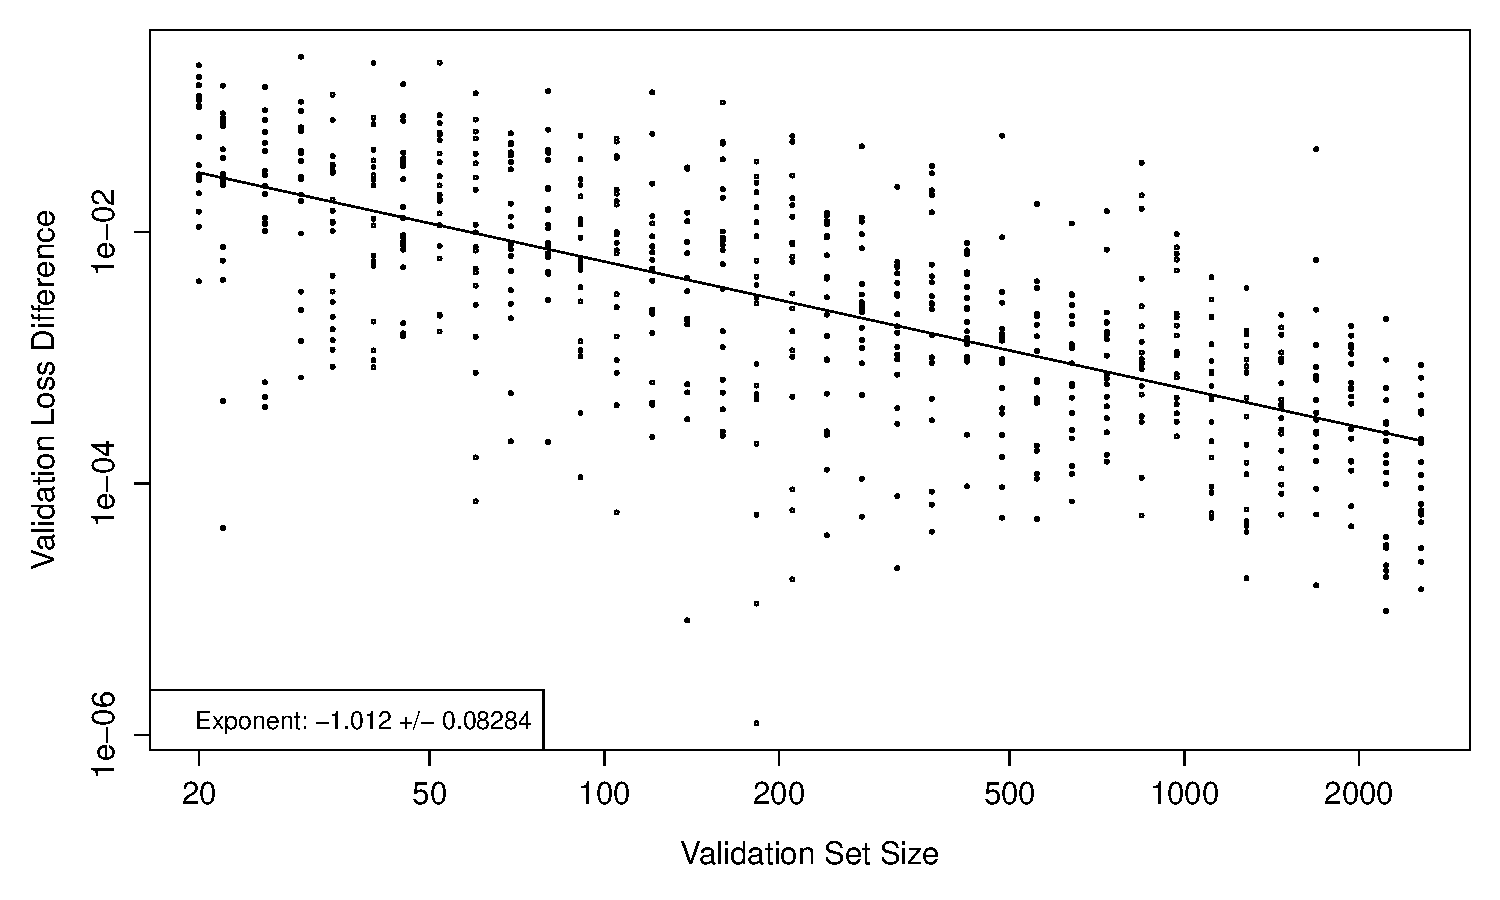
\includegraphics[height=80mm]{../R/figures/validation_size_loss_diff.pdf}
%\includegraphics[height=80mm]{../R/figures/qqplot.pdf}
\end{figure}


\section{Discussion}\label{sec:discussion}

In this paper, we have established oracle inequalities for penalty parameter selection using a training/validation split framework or $k$-fold cross-validation. The results address the concern in \citet{bengio2000gradient} regarding ``the amount of overfitting that can be brought when too many hyperparameters are optimized.'' Our results show that 
this should not be a major concern. In a non-parametric setting or parametric setting where $p$ grows with $n$, the oracle error is the dominating term in the upper bound. At worst, the tuning penalty parameter problem contributes an error that is on the same order as the oracle error, say in a parametric setting where $p$ is fixed. 

There is recent interest in combining regularization methods, but seems to be an artificial restriction to two or three penalty parameters. The area of penalized regression methods with tens or hundreds of penalty parameters remains largely unexplored. Our results suggest that this direction of research could be fruitful. As shown in Feng and Simon (TBD), un-pooling the penalty parameters in a sparse group lasso model is surprisingly effective.

One major caveat to our results is that we have assumed that the penalty parameters can be tuned such that the validation loss is minimized. However it is difficult to find the global minimizer since the validation loss is not convex in the penalty parameters. Optimization methods need to be developed to effectively solve the bilevel optimization problems in \eqref{eq:bilevel}. In addition, it would be worthwhile to understand the performance of models that are only local minimizers of the validation loss.

Finally, there are still many open questions to explore. Our results assume that the fitted models are smoothly parameterized with respect to the penalty parameters and we provide a number of examples that satisfy these conditions. There are probably many more examples of regression problems that satisfy the smoothness condition and the smoothness condition itself can probably be generalized. In addition, it would be interesting to bound the distance between the selected and oracle penalty parameters
\begin{equation}
\label{penalty_diff}
\left \| \hat{\boldsymbol \lambda} - \tilde{\boldsymbol \lambda} \right \|_2
\end{equation}
Such a result would perhaps give a more intuitive understanding of penalty parameter selection methods.


%We find that the difference between the oracle error and the selected model error does not increase dramatically with the number of penalty parameters. the increase in error from tuning parameters model decreases at a near-parametric rate if the fitted models are smoothly parameterized in terms of the penalty parameters. For many penalized regression problems, we find that this is indeed the case. Our results show that adding penalty parameters does not drastically increase the model complexity. This supports recent efforts to combine regularization methods and ``un-pool" regularization parameters. Furthermore, since our result holds for a search over a dense set of penalty parameters, our prediction error bounds apply to cross-validation over a continuum of values, as done in hyper-parameter optimization methods.

\section{The Proof} \label{sec:proofs}

In this paper, we will measure the the complexity of $\mathcal{G}(T)$ by its metric entropy. Let us recall its definition here:

\begin{definition}
Let the covering number $N(u, \mathcal{G}, \| \cdot \|)$ be the smallest set of $u$-covers of $\mathcal{G}$ with respect to the norm $\| \cdot \|$. The metric entropy of $\mathcal{G}$ is defined as the log of the covering number:
\begin{equation}
H (u, \mathcal{G}, \| \cdot \| ) = \log N(u, \mathcal{G}, \| \cdot \|)
\end{equation}
\end{definition}

\begin{theorem}
\label{thrm:train_val_complicated}
\end{theorem}

\begin{theorem}
	\label{thrm:k_fold_complicated}
	This is reproduced from the Mitchell paper
\end{theorem}

\begin{proof}
Chaining and peeling.
\end{proof}


\paragraph{Proof of Theorem \ref{thrm:train_val}}

\begin{proof}

\end{proof}

\paragraph{Proof of Theorem \ref{thrm:kfold}}

%\paragraph{Ridge Perturbations don't change the solution very much - nonsmooth}
%The following lemma considers smooth penalized regression problems; Lemma \ref{lemma:ridge_perturb_nonsmooth} extends it to certain non-smooth problems. (And we don't have anything for nonparametric problems right now)
%\begin{lemma}
%	\label{lemma:ridge_perturb_smooth}
%	Let $L_{T}(\boldsymbol{\theta}|\boldsymbol{\lambda})$ be a training criterion where $\nabla^{2}L_{T}(\boldsymbol{\theta}|\boldsymbol{\lambda})$
%	exists. Suppose $L_{T}(\boldsymbol{\theta}|\boldsymbol{\lambda})$ is $m$-strongly convex in $\boldsymbol{\theta}$:
%	$$
%	\nabla^{2}L_{T}(\boldsymbol{\theta})\succeq mI
%	$$
%	
%	Let
%	\begin{equation}
%	\hat{\boldsymbol{\theta}}_{\boldsymbol{\lambda}}(w)=\arg\min_{\theta}L_{T}(\boldsymbol{\theta})+\sum_{j=1}^{J}\lambda_{j}\frac{w}{2}\|\boldsymbol{\theta}\|^{2}
%	\end{equation}
%	
%	For any $w>0$, we have
%	\begin{equation}
%	\left \|
%	\hat{\boldsymbol{\theta}}_{\boldsymbol{\lambda}}(w)-\hat{\boldsymbol{\theta}}_{\boldsymbol{\lambda}}(0)
%	\right \|_{2}	
%	\le	
%	2 \frac{w}{m} \left(\sum_{j=1}^{J}\lambda_{j}\right)
%	\left \|\hat{\boldsymbol{\theta}}_{\boldsymbol{\lambda}}(0) \right \|
%	\end{equation} 
%	
%\end{lemma}

\paragraph{Proof of Lemma \ref{lemma:param_add}}

\paragraph{Proof of Lemma \ref{lemma:nonsmooth}}

\paragraph{Proof of Lemma \ref{lemma:nonparam_smooth}}


\bigskip

\bibliographystyle{agsm}
\bibliography{multi-penalties-theory}

\end{document}
